\documentclass[]{article}
\newcommand{\FileDepth}{../../..}
\usepackage[letterpaper, landscape, margin=0.5cm]{geometry}
\usepackage[T1]{fontenc}
\usepackage{textcomp}%Not strictly necessary, but gives \textmu command for "micro."
\usepackage{fancyhdr}
\usepackage{amsmath}
\usepackage{amssymb}
\usepackage{graphicx}
\usepackage{xcolor}
\usepackage{tikz}
\usetikzlibrary{calc}
\usepackage[shortlabels]{enumitem}
\usepackage{multicol}
\usepackage{vwcol}
\usepackage{hyperref}
\usepackage{wrapfig}
%opening
\newcommand{\SecType}{L}
\newcommand{\Week}{16}
\title{PH 211 Lecture \Week}
\author{Benjamin Bauml}
\date{Summer 2024}

\newcommand{\Purpose}{4}
\newcommand{\DefOnly}{0}

% Version 2024-06-14
% Changes
% 2024-02-21 Added xstring package to enable smooth implementation of new \ModePage command.
% 2024-04-27 Set up to split activities and formatting aspects into separate files. Removed dependence on xcomment. Added an automatic counter to number the activities in a problem set.
% 2024-05-19 Revised old format for \TeachingTips command, which did not support \DefOnly.
% 2024-06-14 Added Repurpose environment to allow mixing of different purpose levels in the same document.
\usepackage{tcolorbox}
\usepackage{xstring}
% You will want the following four lines in your document (the last two uncommented):
% For Assignment, leave Purpose as 1. For Worksheet, set to 2. For Student Solution, set to 3. For Teacher Solution, set to 4.
% If you want keep the pieces from being called manually, set DefOnly to 0.
%\newcommand{\Purpose}{4}
%\newcommand{\DefOnly}{1}
\newcommand{\Exclusion}{0}
\newcommand{\PageTurn}{0}
\newcommand{\GrayProb}{0}
\newcommand{\Tipsy}{0}

% Assignment
\if\Purpose1
\renewcommand{\Exclusion}{1}
\fi
% Worksheet
\if\Purpose2
\renewcommand{\Exclusion}{1}
\renewcommand{\PageTurn}{1}
\fi
% Student Solution
\if\Purpose3
\renewcommand{\PageTurn}{1}
\renewcommand{\GrayProb}{1}
\fi
% Teaching Copy
\if\Purpose4
\renewcommand{\PageTurn}{1}
\renewcommand{\GrayProb}{1}
\renewcommand{\Tipsy}{1}
\fi

\newenvironment{Repurpose}[1]{
\renewcommand{\Purpose}{#1}
\renewcommand{\Exclusion}{0}
\renewcommand{\PageTurn}{0}
\renewcommand{\GrayProb}{0}
\renewcommand{\Tipsy}{0}
% Assignment
\if\Purpose1
\renewcommand{\Exclusion}{1}
\fi
% Worksheet
\if\Purpose2
\renewcommand{\Exclusion}{1}
\renewcommand{\PageTurn}{1}
\fi
% Student Solution
\if\Purpose3
\renewcommand{\PageTurn}{1}
\renewcommand{\GrayProb}{1}
\fi
% Teaching Copy
\if\Purpose4
\renewcommand{\PageTurn}{1}
\renewcommand{\GrayProb}{1}
\renewcommand{\Tipsy}{1}
\fi
}{}

\def \NewQ {0}
\def \PForce {0}
\newcommand{\MaybePage}[1]{
	\def \PForce {#1}
	\if\PForce1
	\newpage
	\else
	\if\NewQ0
	\gdef \NewQ {\PageTurn}
	\else
	\newpage
	\fi
	\fi
}

\newcommand{\ModePage}[1]{
	\IfSubStr{#1}{\Purpose}{\newpage}{}
}

\newcounter{ActNumber}
\setcounter{ActNumber}{0}

\newcommand{\Problem}[4][0]{%The first argument is optional, and if it is set to 1, the \newpage will be forced. The second argument is the name of the activity, the third is the command the activity is stored as, and the fourth is the actual problem statement.
\newcommand{#3}{
\MaybePage{#1}
\addtocounter{ActNumber}{1}
\section*{\SecType\Week-\theActNumber: #2}
\if\GrayProb1
\begin{tcolorbox}[colback=lightgray,colframe=lightgray,sharp corners,boxsep=1pt,left=0pt,right=0pt,top=0pt,bottom=0pt,after skip=2pt]
\else
\begin{tcolorbox}[colback=white,colframe=white,sharp corners,boxsep=1pt,left=0pt,right=0pt,top=0pt,bottom=0pt,after skip=2pt]
\fi
#4
\end{tcolorbox}\noindent
}
\if\DefOnly0
\else
#3
\fi
}
	
\newcommand{\ProblemSub}[3][0]{%The first argument is optional, and if a string of numbers is entered into it, it will force a \newpage in any \Purpose that shows up in the string. For example, "13" would lead to the newpage being forced in modes 1 and 3. The second is the command the activity is stored as, and the third is the actual problem statement.
\newcommand{#2}{
\ModePage{#1}
\if\GrayProb1
\begin{tcolorbox}[colback=lightgray,colframe=lightgray,sharp corners,boxsep=1pt,left=0pt,right=0pt,top=0pt,bottom=0pt,after skip=2pt]
\else
\begin{tcolorbox}[colback=white,colframe=white,sharp corners,boxsep=1pt,left=0pt,right=0pt,top=0pt,bottom=0pt,after skip=2pt]
\fi
#3
\end{tcolorbox}\noindent
}
\if\DefOnly0
\else
#2
\fi
}
		
\newcommand{\Solution}[2]{%The first argument is the command the solution is stored as, and the second is the actual solution.
\newcommand{#1}{
\if\Exclusion0
#2
\fi
}
\if\DefOnly0
\else
#1
\fi
}
		
\newcommand{\ProblemFig}[2]{%The first argument is the command the figure is stored as, and the second is the actual figure.
\newcommand{#1}{
\begin{figure}[h]
#2
\end{figure}
}
\if\DefOnly0
\else
#1
\fi
}

\newcommand{\TeachingTips}[2]{%The first argument is the command the tip is stored as, and the second is the actual tip.
\newcommand{#1}{
\if\Tipsy1
\begin{tcolorbox}[colback=lightgray,colframe=black]
#2
\end{tcolorbox}
\fi
}
\if\DefOnly0
\else
#1
\fi
}
\usepackage[absolute]{textpos}
% This package relies on Assignment Format 2024-06-14 or later to work. It is recommended that the Purpose and DefOnly commands be given as such:
%\newcommand{\Purpose}{4}
%\newcommand{\DefOnly}{0}
% Activities need to be entered outside of the TeacherMargin and PresentSpace environments, otherwise they will be defined only locally. They can even go in the preamble.
\newenvironment{TeacherMargin}{\begin{textblock*}{10.8cm}(0.5cm,0.5cm)
\small}{\end{textblock*}
\hspace{0.1cm}}
\newenvironment{PresentSpace}{\begin{textblock*}{0.3cm}(26.85cm,9.35cm)
--
\end{textblock*}
\begin{textblock*}{0.3cm}(26.85cm,18.7cm)
--
\end{textblock*}
\begin{textblock*}{0.3cm}(26.85cm,12.24cm)
	--
\end{textblock*}
\begin{textblock*}{15.6cm}(11.8cm,0.5cm)
\begin{Repurpose}{1}
\Large}{\end{Repurpose}
\end{textblock*}
\hspace{0.1cm}}

\newcommand{\FBDaxes}[3]{
	\begin{scope}[shift={(#1)},rotate=#2]
		% x-axis
		\draw[thick,->] (-2,0) -- (2,0);
		\node[anchor=west] at (2,0) {$x$};
		% y-axis
		\draw[thick,->] (0,-2) -- (0,2);
		\node[anchor=west] at (0,2) {$y$};
		\coordinate (#3) at (0,0);
	\end{scope}
}
\newcommand{\FBDvectorMA}[4]{
	\begin{scope}[shift={(#1)}]
		\coordinate (#4tip) at ({#2*cos(#3)},{#2*sin(#3)});
		\draw[ultra thick,blue,->] (#1) -- (#4tip);
	\end{scope}
}
\newcommand{\FBDvectorXY}[3]{
	\begin{scope}[shift={(#1)}]
		\coordinate (#3tip) at (#2);
		\draw[ultra thick,blue,->] (0,0) -- (#3tip);
	\end{scope}
}
\newcommand{\FBDdot}[1]{
	\filldraw[black] (#1) circle (3pt);
}
%\newcommand{\MVec}[3][0]{%Creates a momentum vector of length #3 centered at #2 and rotated #1 degrees counterclockwise.
	\begin{scope}[rotate=#1,shift={(#2)}]
		\draw[->,thick] ({-#3/2},0) -- ({#3/2},0);
	\end{scope}
}
\newcommand{\MDot}[1]{%Creates a dot at #1 to represent a zero vector.
	\filldraw (#1) circle (1pt);
}
\newcommand{\MVDRows}[2][4.5]{%Creates the rows (initial, delta, final) of a momentum vector diagram. The optional argument determines the width of the table, and defaults to a good length for three columns (two objects and the total system). The non-optional argument gives a coordinate name (not displayed) to the diagram.
	\begin{scope}
		%\draw[thick] (0,5.5) -- (0,0);
		\draw[thick] (-1,4.5) -- (#1,4.5);
		\node at (-0.5,3.75) {$\vec{p}_{i}$};
		\draw[thick] (-1,3) -- (#1,3);
		\node at (-0.5,2.25) {$\Delta\vec{p}$};
		\draw[thick] (-1,1.5) -- (#1,1.5);
		\node at (-0.5,0.75) {$\vec{p}_{f}$};
		\coordinate (#2) at (0,5);
	\end{scope}
}
\newcommand{\MVDCol}[4][0.75]{%Creates a column for an object in a momentum vector diagram. The first (non-optional) argument is the coordinate name (not displayed) of the column, while the second is the displayed column header. The first argument also names the three entries down the column. The third argument anchors the column, so it should either be the coordinate name of the MVD (for the first column) or the coordinate name of the previous column. The optional argument indicates how far the center of the column should be from the previous column's edge, and defaults to 0.75
	\begin{scope}[shift={(#4)}]
		\node at (#1,0) {#3};
		%\draw[thick] ({#1*2},0.5) -- ({#1*2},-5);
		\draw[thick] (0,0.5) -- (0,-5);
		\coordinate (#2init) at (#1,-1.25);
		\coordinate (#2delt) at (#1,-2.75);
		\coordinate (#2fin) at (#1,-4.25);
		\coordinate (#2) at ({#1*2},0);
	\end{scope}
}

%\input{\FileDepth/Activities/Activity_One/Activity_One.tex}
%\input{\FileDepth/Activities/Activity_Two/Activity_Two.tex}

\begin{document}
\begin{TeacherMargin}

\end{TeacherMargin}
\begin{PresentSpace}
\begin{center}
	\huge Lecture \Week: Power
\end{center}
\vspace{0.5cm}
\underline{Announcements}
\begin{itemize}
	\item Homework \textbf{and} Get-Ready Assignments on Gradescope
	\begin{itemize}
		\item Regrade requests can be used to ask for clarification on feedback you have received.
		\item This week's homework is long, in order to keep next week's homework shorter.
	\end{itemize}
	\item Project Peer Review
	\begin{itemize}
		\item Complete your feedback by Friday at the latest.
		\item Please offer criticisms with care and respect; you are trying to help your peers improve their work.
		\item You should write 1-2 paragraphs for each peer review.
		\item Point out things that were done well, and things that can be improved.
		\begin{itemize}
			\item Giving positive comments on what works and should be kept is just as important as suggesting revisions and giving constructive criticism.
		\end{itemize}
		\item Scientific communication is a major goal of this work, so don't be shy about asking (nicely) for things to be explained better.
		\begin{itemize}
			\item If you don't understand something, don't be shy about admitting it.
			\item If you do understand something, but think it could be explained better, remark on this as well.
		\end{itemize}
	\end{itemize}
\end{itemize}
\end{PresentSpace}
\newpage
\begin{TeacherMargin}

\end{TeacherMargin}
\begin{PresentSpace}
\vspace{-10pt}
\section*{A Deeper Model for Interactions}
\vspace{-10pt}
\begin{itemize}
	\item Quantities
	\begin{itemize}
		\item Energy \qquad \qquad \qquad \quad \ \ $E$
		\item Kinetic Energy \qquad \qquad $K=\frac{1}{2}mv^{2}$
	\end{itemize}
	\item Laws
	\begin{itemize}
		\item Work-energy theorem \quad $W_{\text{net,ext}} = \Delta E_{\text{total}}$
	\end{itemize}
\end{itemize}
\end{PresentSpace}
\newpage
\begin{TeacherMargin}

\end{TeacherMargin}
\begin{PresentSpace}
\vspace{-10pt}
\section*{Power}
\vspace{-10pt}
\begin{itemize}
	\item When the energy of a system changes, we sometimes want to know how \textit{fast} it changes.
	\item \textit{Power} is the time rate of change of energy:
	\[
	P=\frac{dE}{dt}.
	\]
	\item Power is measured in watts (W).
\end{itemize}
\end{PresentSpace}
\newpage
\begin{TeacherMargin}
\begin{center}
	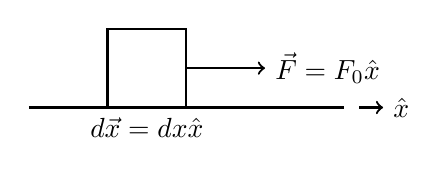
\begin{tikzpicture}
		\draw[thick] (0,0) -- (4,0);
		\draw[thick,->] (4.2,0) -- (4.5,0) node[anchor=west] {$\hat{x}$};
		\node[anchor=north] at (1.5,0) {$d\vec{x} = dx\hat{x}$};
		\draw[thick] (1,0) rectangle (2,1);
		\draw[thick,->] (2,0.5) -- (3,0.5) node[anchor=west] {$\vec{F} = F_{0}\hat{x}$};
	\end{tikzpicture}
\end{center}
\textbf{Total Energy} \\
The block can have kinetic energy, so its change in total energy is the difference of its final and initial kinetic energies. Its initial speed is 0 m/s, so
\[
\Delta E = K_{f}-K_{i} = \frac{1}{2}mv_{f}^{2} - \frac{1}{2}mv_{i}^{2} = \frac{1}{2}mv_{f}^{2}.
\]
Plugging in numbers, we obtain $\Delta E = 9000$ J. \\
\textbf{Distance} \\
By the work-energy theorem, $W_{\text{net,ext}} = \Delta E$, so if there is no friction and the winch is the only thing doing work, then we can calculate the distance $d$ from the work it did:
\[
W = \int_{0}^{d}\vec{F}\cdot d\vec{x} = F_{0} d = \Delta E = \frac{1}{2}mv_{f}^{2}.
\]
Solving for $d$ gives us $d = \frac{m}{2F_{0}}v_{f}^{2}$, and plugging in numbers gives us $d = 0.5$ m. \\
\textbf{Power} \\
We know how much energy the winch put into this endeavor, so all we need to find out is the time it took to move the block. For constant acceleration (which we have in this situation of constant force), we know $a = \frac{\Delta v}{\Delta t} = \frac{F_{0}}{m}$, so $\Delta t = \frac{v_{f}m}{F_{0}} = \frac{1}{6}$ s. This means that the power is
\[
P = \frac{\Delta E}{\Delta t} = \frac{F_{0}d}{v_{f}m/F_{0}} = \frac{F_{0}^{2}d}{v_{f}m}.
\]
Given what we know about the distance, this simplifies to
\[
P = \frac{F_{0}^{2}}{v_{f}m}\frac{m}{2F_{0}}v_{f}^{2} = \frac{F_{0}v_{f}}{2} = 54,000\text{ W}.
\]
For comparison, the light bulb in my desk lamp in my apartment consumes 9 W while on (this is much more efficient than an equivalently bright incandescent bulb, which would take about 60 W). This much power could light 6,000 desk lamps (or 900 if using an incandescent bulb)!
\end{TeacherMargin}
\begin{PresentSpace}
\vspace{-10pt}
\section*{L\Week-1: The Winch -- Part 1}
\vspace{-10pt}
A winch acts a constant force $F_{0}=18,000$ N on a metal block ($m=500$ kg) to accelerate it across level ground from rest to a final speed of $v_{f}=6$ m/s.
\begin{itemize}
	\item What is the block's change in total energy?
	\item How far did the winch move the block?
	\item How much power does this winch use?
\end{itemize}
\end{PresentSpace}
\newpage
\begin{TeacherMargin}
\noindent\textbf{Force} \\
To keep the block at constant speed, the winch must exert a force equal in magnitude to the force of gravity on the block:
\begin{center}
	\begin{tikzpicture}
		\FBDbox{0,0}{0}{block}{500 kg}
		\FBDvectorXY{blocktcent}{0,1}{FT}
		\node[anchor=south] at (FTtip) {$\vec{F}^{T}$};
		\FBDvectorXY{blockbcent}{0,-1}{FG}
		\node[anchor=north] at (FGtip) {$\vec{F}^{g}$};
	\end{tikzpicture}
\end{center}
\[
F^{T} = F^{g} = mg \approx (500\text{ kg})(10\text{ m/s}^{2}) = 5000\text{ N}
\]
\textbf{Distance Lifted} \\
We know the speed of the block and how long it is in motion, so we can calculate its displacement directly from this:
\[
\Delta y = v\Delta t = (2\text{ m/s})(30\text{ s}) = 60\text{ m}.
\]
\textbf{Work}
\begin{align*}
	W & = \int_{y_{i}}^{y_{f}}\vec{F}\cdot d\vec{y} = \int_{y_{i}}^{y_{f}}\left(F\hat{y}\right)\cdot\left(dy\hat{y}\right) = \int_{y_{i}}^{y_{f}}Fdy \\
	& = F\Delta y = (5000\text{ N})(60\text{ m}) = 300,000\text{ J}
\end{align*}
Note that the speed is not changing, so the total energy of the block is not changing. That means $W_{\text{net,ext}}=\Delta E_{\text{total}} = 0$. Something else must be doing work to remove energy from the system! This is being done by gravity. \\
\textbf{Power} \\
The winch is transferring 300,000 J of energy over the course of 30 s, so the power is
\[
P = \frac{\Delta E}{\Delta t} = \frac{300,000\text{ J}}{30\text{ s}} = 10,000\text{ W}.
\]
This much power could light about 1,111 desk lamps (or about 166 if using an incandescent bulb)!
\end{TeacherMargin}
\begin{PresentSpace}
\vspace{-10pt}
\section*{L\Week-1: The Winch -- Part 2}
\vspace{-10pt}
You want to use the winch to lift the block into the air at a constant speed: $v=2$ m/s.
\begin{itemize}
	\item What force should you set the winch for?
	\item How far does the winch move the block from $t=0$ s to $t=30$ s?
	\item How much work does the winch do in $\Delta t = 30$ s?
	\begin{itemize}
		\item Is anything else doing work on the block?
	\end{itemize}
	\item How much power does the winch use now?
\end{itemize}
\end{PresentSpace}
\newpage
\begin{TeacherMargin}

\end{TeacherMargin}
\begin{PresentSpace}
\vspace{-10pt}
\section*{Energy Analysis}
\vspace{-10pt}
\begin{itemize}
	\item Understanding: Identify a system and the types of energy within the system.
	\item Calculating: Is your system's energy conserved or not? Once you know, use the work-energy theorem!
	\item Sensemaking: All the sensemaking strategies you have will work, but a new strategy is sometimes useful: Solve Multiple Ways.
	\begin{itemize}
		\item You have kinematics and force techniques at your disposal, so you can solve problems with these and compare their results to the results of your energy approach.
	\end{itemize}
\end{itemize}
\end{PresentSpace}
\newpage
\begin{TeacherMargin}

\end{TeacherMargin}
\begin{PresentSpace}
\section*{Main Ideas}
\begin{itemize}
	\item Energy is a powerful, ubiquitous concept that can help us solve a wide array of physics problems.
	\item Energy is a \textit{scalar}---it is not a vector.
	\item There are different forms of energy, and energy can be transferred between objects and between forms.
\end{itemize}
\end{PresentSpace}
\end{document}